\chapter{Introduction}

This document is designed to be a gentle introduction to programming
with the NASA Vision Workbench, a C++ image processing and machine
vision library.  The Vision Workbench was developed through a joint
effort of the Intelligent Robotics Group (IRG) and the Adaptive
Control and Evolvable Systems Group (ACES) within the Intelligent
Systems Division at the NASA Ames Research Center in Moffett Field,
California.  It is distributed under the NASA Open Source Agreement
(NOSA) version 1.3, which has been certified by the Open Source
Initiative (OSI).  A copy of this agreement is included with every
distribution of the Vision Workbench in a file called {\tt COPYING}.

You can think of the Vision Workbench as a ``second-generation'' C/C++
image processing library.  It draws on the authors' experiences over
the past decade working with a number of ``first-generation''
libraries, such as OpenCV and VXL, as well as direct implementations
of image processing algorithms in C.  We have tried to select and
improve upon the best features of each of these approaches to image
processing, always with an eye toward our particular range of NASA
research applications.  The Vision Workbench has been used within NASA
for a wide range of image processing tasks, including alignment and
stitching of panoramic images, high-dynamic-range imaging, texture
analysis and recognition, lunar and planetary map generation, and the
production of 3D models from stereo image pairs.  A few examples of
image data that has been processed with the Vision Workbench are show
in Figure~\ref{fig:examples}.

\begin{figure}[p]
\centering
  \subfigure[]{\hbox{\hspace{0.25in}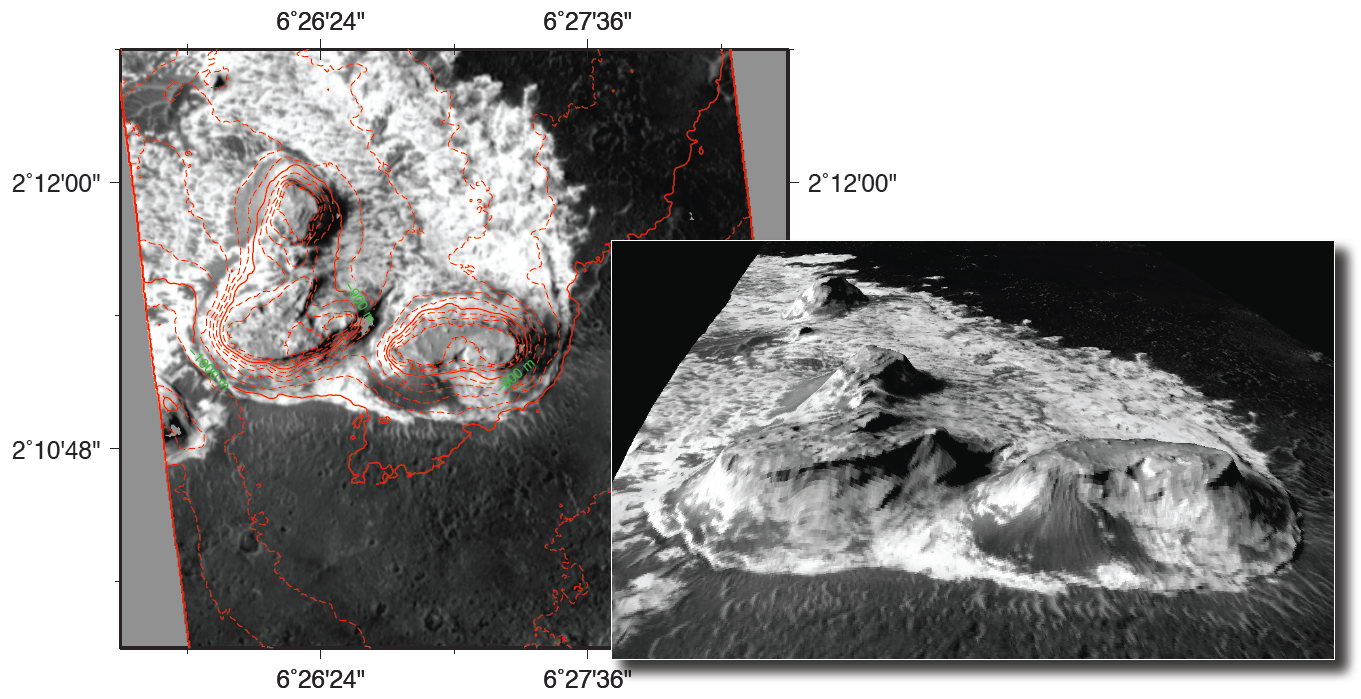
\includegraphics[width=5in]{images/mars_dem.png}\hspace{0.25in}\ \label{fig:examples.marsdem}}}
  \\
  \subfigure[]{\hbox{\hspace{0.25in}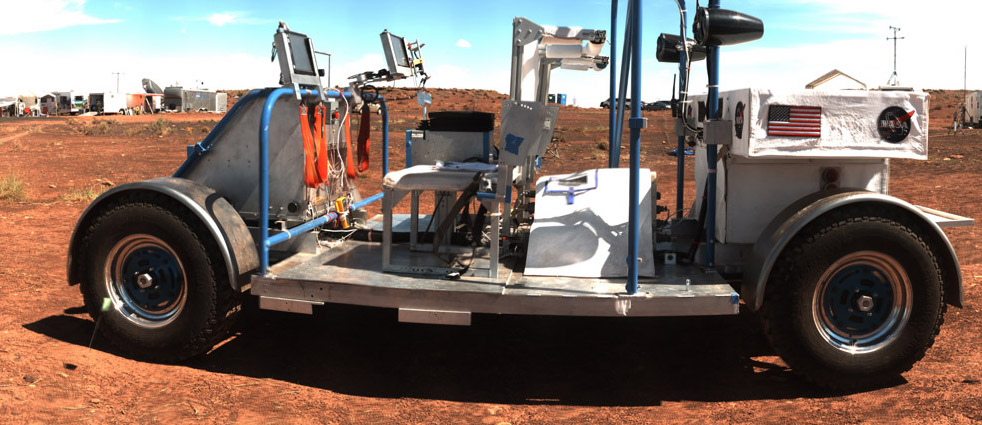
\includegraphics[width=2.75in]{images/scout_ldr.jpg}\hspace{0.25in}\ \label{fig:examples.scoutldr}}}
  \hfil
  \subfigure[]{\hbox{\hspace{0.25in}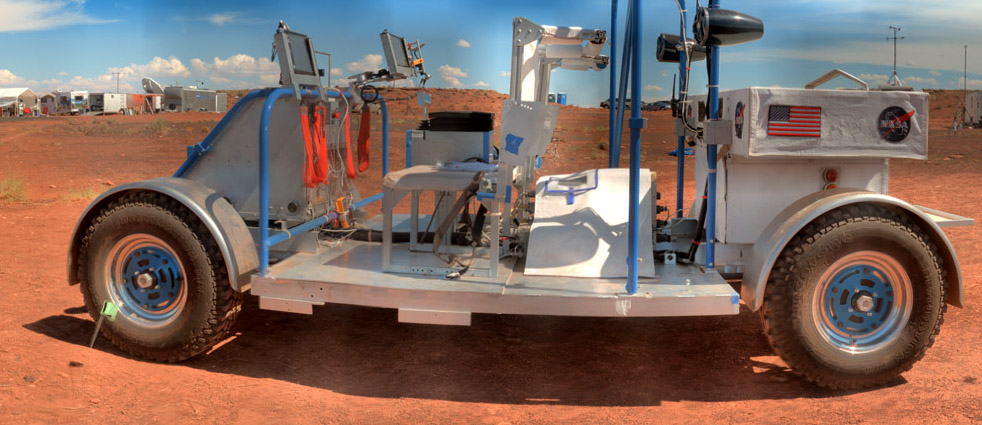
\includegraphics[width=2.75in]{images/scout_hdr.jpg}\hspace{0.25in}\ \label{fig:examples.scouthdr}}}
  \\
  \subfigure[]{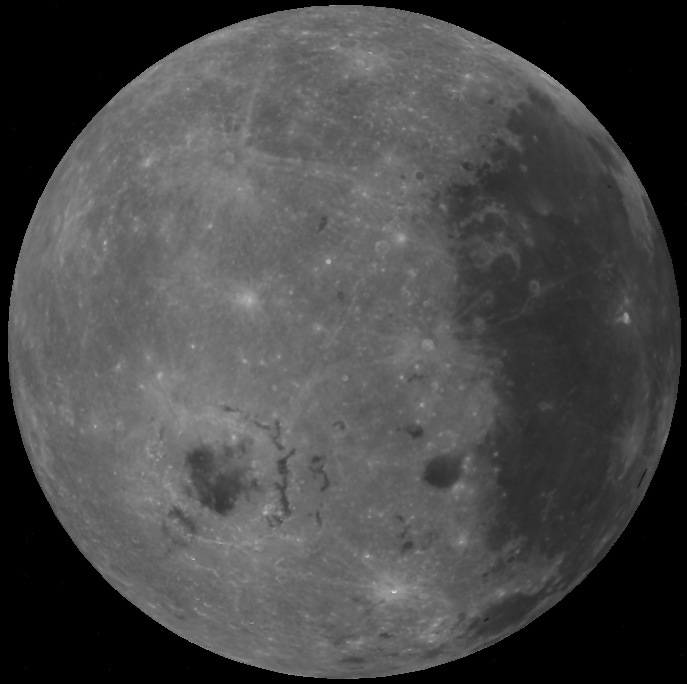
\includegraphics[width=2.5in]{images/moon_sphere.jpg}\label{fig:examples.moon}}
\caption{Examples of image data processed with the help of the Vision Workbench.  (a) A Martian terrain map generated from 
stereo satellite imagery.  (b,c) Original and high-dynamic-range image mosaics from a NASA field test.  (d) A lunar 
base map generated from the Clementine data set. }
\label{fig:examples}
\end{figure}

The Vision Workbench was designed from the ground up to make it quick
and easy to produce efficient implementations of a wide range of image
processing algorithms.  Consider this example:
\begin{verbatim}
  background_image += 0.1 * ( source_image - background_image );
\end{verbatim}
Hopefully it is reasonably clear what this line of code does, even 
if you don't know what an IIR filter like this is good for.  Higher 
level functions have similarly simple interfaces.  For example, to 
apply a Gaussian filter to an image with a sigma of 3 pixels you 
can simply say:
\begin{verbatim}
  image = gaussian_filter( image, 3 );
\end{verbatim}
In many cases like these, code written using the Vision Workbench is
significantly smaller and more readable than code written using more
traditional approaches.

At the core of the Vision Workbench is a rich set of template-based
image processing data types representing pixels, images, and
operations on those images, as well as mathematical entities (like
vectors and geometric transformations) and image file I/O.  On top of
this core the Vision Workbench also provides a number of higher-level
image processing and machine vision modules, providing features
including camera geometry modeling, high-dynamic-range imaging,
interest point detection and matching, image mosaicing and blending,
and geospatial data management.

That said, the Vision Workbench is not for everyone, and in particular
it is not intended as a drop-in replacement for any existing image
processing toolkit.  It is specifically designed for image processing
in the context of machine vision, so it lacks support for things like
indexed color palettes that are more common in other areas.  It also
lacks a number of common features that the authors have simply not yet
had a need for, such as morphological operations.  If you encounter one
of these holes while using the Vision Workbench please let us know: if
it is an easy hole to fill we may be able to do so quickly.  Finally,
there are many application-level algorithms, such as face recognition,
that have been implemented using other computer vision systems and are
not currently provided by the Vision Workbench.  If one of these meets
your needs there is no compelling reason to re-implement it using the
Vision Workbench instead.  On the other hand, if no existing
high-level tool solves your problem then you may well find that the
Vision Workbench provides the most productive platform for developing
something new.

Since this is the first public release of the Vision Workbench, we
thought we should also provide you with some sense of the direction
the project is headed.  It is being actively developed by a small but
growing team at the NASA Ames Research Center.  A number of features
are currently being developed internally and may released in the
future, including improved mathematical optimization capabilities, a
set of Python bindings, and stereo image processing tools. Development
of the code can be seen on our GitHub account under the username
\verb#visionworkbench#. If you have feature requests, suggestions, or
bug reports please let us know through GitHub. You are also encourage
to fork our repository and to produce your own modifications.

We hope that you enjoy using the Vision Workbench as much as we have
enjoyed developing it!  If you have any questions, suggestions,
compliments or concerns, please let us know.  Contact information is
available at the bottom of the \verb#README# file included with your
distribution.
